Parmi les trois étapes constitutives de la phase de décomposition,
seule la décomposition des \emph{relations de localisation} nécessite
le développement d'une méthode spécifique. En effet, les étapes de
décomposition de ensemble des \emph{indices de localisation} et des
\emph{objets de référence indéfinis} ne font qu'expliciter un
découpage présent dès la saisie. Ces deux opérations ne nécessitent
donc pas l'apport de connaissances supplémentaires, contrairement à la
décomposition des \emph{relations de localisation.}

En effet, les \emph{principes de décomposition} et de
\texttt{intégration contexte métier} s'opposent en partie. Si la
décomposition permet de faciliter la \emph{spatialisation} des
\emph{indices de localisation} en permettant de manipuler des concepts
précis et en minimisant les redondances, elle implique également de
travailler à l'aide de \emph{relations de localisation} (atomiques)
\emph{ad hoc,} qui ne sont pas destinées à être manipulées directement
par l'utilisateur. Il est donc inenvisageable de demander à
l'utilisateur de saisir des \emph{relations de localisation
  atomiques,} qui ne sont pas prévues pour. C'est pourquoi nous
proposons d'automatiser cette étape.

\subsection{La décomposition des \emph{relations de localisation}}

Nous avons précédemment abordé la décomposition des \emph{relations de
  localisation} en la présentant comme le processus permettant de
passer d'une \emph{relation de localisation} à un ensemble de
\emph{relations de localisations atomiques} liées par des conjonctions
et auxquelles est apposée une méthode de \emph{spatialisation,}
permettant de construire la \emph{zone de localisation compatible}
correspondant à la \emph{relation de localisation atomique} pour un
\emph{objet de référence} donné. La difficulté majeure de cette
décomposition consiste donc à identifier la manière dont les
\emph{relations de localisation} utilisées par le requérant se
décomposent. Notre objectif étant de proposer une décomposition selon
des critères sémantiques, propres à chaque \emph{relation de
  localisation,} il est nécessaire de disposer de connaissances à
priori sur la sémantique des \emph{relations de localisation.} Nous
proposons donc de créer une base de règles, formalisant la
décomposition de chaque \emph{relation de localisation} en des
\emph{relations de localisation atomiques} spatialisables. Ce qui
permettrait de décomposer les \emph{relations de localisation} avec une
méthode en trois étapes :
%
\begin{enumerate*}[label=(\arabic*)] 
\item réception de la \emph{relation de localisation}
  $\text{\textsf{rl}}$ à décomposer,
\item lecture de la base de règles et identification des règles
  définies pour la \emph{relation de localisation}
  $\text{\textsf{rl}}$ et
\item application des règles de décomposition à la \emph{relation de
    localisation} $\text{\textsf{rl}}$.
\end{enumerate*}
%
Ce processus de décomposition, illustré par la
\autoref{fig:logique_dec}, nécessite donc deux entrées : une
\emph{relation de localisation} à décomposer et une base de règles,
définissable en amont et qui ne sera modifiée que lorsque nécessaire
(\eg correction d'erreurs, ajustement, ajout de nouvelles règles,
\emph{etc.})

La constitution d'une telle base pose cependant plusieurs problèmes,
que ce soit au niveau de la définition de sa structure ou de son
contenu. Il est en effet nécessaire qu'elle permette de formaliser
toutes les variations de décompositions souhaitées, qu'il faut alors
identifier. De plus, cette organisation ne permet de décomposer que
des \emph{relations de localisation} incluses dans la base de
règles. Il est donc indispensable qu'elle contienne l'ensemble des
\emph{relations de localisation} pertinentes dans notre contexte et
leur décomposition. La constitution d'une telle base de règles
nécessite donc au préalable un travail d'identification et de
définition des \emph{relations de localisations} utilisées dans notre
contexte.

\begin{figure}
  \centering
  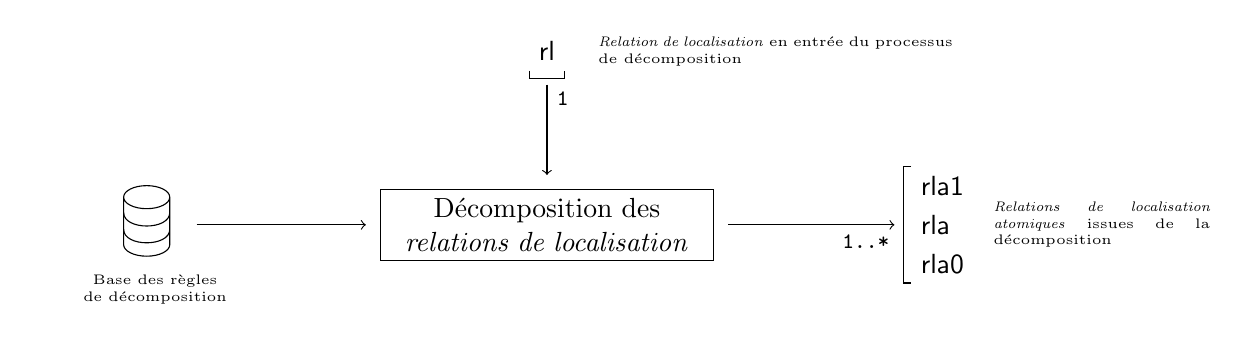
\begin{tikzpicture}
  \usetikzlibrary{shapes.geometric}
  
  \tikzset{
    database/.style={cylinder,aspect=0.5,draw,rotate=90,path picture={
        \draw (path picture bounding box.160) to[out=180,in=180] (path picture bounding
        box.20);
        \draw (path picture bounding box.200) to[out=180,in=180] (path picture bounding
        box.340);
      }
    }
  }
  % 
  \node[text width=4cm, align=center, draw] (dec) {Décomposition des
    \emph{relations de localisation}};
  % 
  \node[anchor=south,above=1.5cm of dec] (rl) {$\text{\textsf{rl}}$};
  % 
  \node[anchor=east, left=2.5cm of dec] (db) {};
  % 
  \node[database, scale=2.5] at ([xshift=-6,yshift=-3]db.west) {};
  % 
  \node[align=center, text width=3cm, font=\tiny] at
  ([xshift=-3,yshift=-.7cm]db.south west) {Base des règles de
    décomposition};
  % 
  \node[anchor=west, right=2.5cm of dec] (rla)
  {$\text{\textsf{rla}}$};
  % 
  \node[anchor=north west] (rla0) at (rla.south west)
  {$\text{\textsf{rla0}}$};
  % 
  \node[anchor=south west] (rla1) at (rla.north west)
  {$\text{\textsf{rla1}}$};
  % 
  \node[anchor=west,align=justify, text width=2.75cm, font=\tiny] at
  ([xshift=2ex]rla.east) {\emph{Relations de localisation atomiques}
    issues de la décomposition};
  % 
  \node[anchor=west,align=justify, text width=4.5cm, font=\tiny] at
  ([xshift=2ex]rl.east) {\emph{Relation de localisation} en entrée du
    processus de décomposition};
  % 
  % Accolades
  \draw (rl.south west) |-
  ($(rl.south west)!0.5!(rl.south east) + (0,-.1)$) -| (rl.south east)
  node[pos=0, yshift=.2] (I-p) {};
  % 
  \draw (rla1.north west) -|
  ($(rla1.north west)!0.5!(rla0.south west) + (-.1,0)$) |- (rla0.south west)
  node[pos=0, yshift=.2] (I-p) {};
  % Arrows
  \draw[->, shorten >=5pt,shorten <=5pt] (rl.south) -- (dec.north)
  node[pos=0,below
  right,yshift=-.15cm,font=\footnotesize\ttfamily]{1};
  % 
  \draw[->, shorten >=5pt,shorten <=5pt] (db.east) -- (dec.west);
  % 
  \draw[->, shorten >=6pt,shorten <=5pt] (dec.east) -- (rla.west) node[pos=1,below
  left,xshift=-.15cm,font=\footnotesize\ttfamily]{1..*};
\end{tikzpicture}
  \caption{Illustration du processus de décomposition des relations de
  localisation}
  \label{fig:logique_dec}
\end{figure}

Dans le cas qui nous a servi à présenter le \emph{principe de
  décomposition} (cf. \autoref{chap;04}) une \emph{relation de
  localisation} (\enquote{sous}) était décomposée en deux
\emph{relations de localisation atomiques} (\enquote{proche} et
\enquote{altitude inférieure}). Si cette configuration a pour mérite
de bien illustrer le fonctionnement et l'objectif du \emph{principe de
  décomposition,} elle ne présente qu'une des configurations
possibles. Tout d'abord il est possible qu'une \emph{relation de
  localisation} soit décomposable en plus de deux \emph{relations de
  localisations.} Par exemple, \textcite{Vanegas2011}, proposent de
décomposer la \emph{relation de localisation} \enquote{entouré de}
(dans \emph{l'indice de localisation} \enquote{A est entouré de B}),
avec des \emph{relations de localisation} directionnelles, donnant les
\emph{indices de localisation:} \enquote{B est au nord de A},
\enquote{B est à l'est de A}, \enquote{B est au sud de A} et
\enquote{B est à l'ouest de A}. Ainsi, il n'y a aucune raison à
limiter le nombre de \emph{relations de localisation atomiques}
décomposant une \emph{relation de localisation,} même s'il est peu
probable que se nombre puisse atteindre des très grandes valeurs. À
l'inverse, on peut se questionner sur la possibilité que certaines
\emph{relations de localisation} ne soient pas décomposables. Par
exemple, la \emph{relation de localisation} \enquote{à} (\eg je suis
au sommet) ne nous semble pas décomposable, pourtant il s'agit bien
d'une \emph{relation de localisation,} que l'on est amené à utiliser
fréquemment. Dans ce cas, \emph{relation de localisation} et
\emph{relation de localisation atomique} sont confondues. Cet exemple
illustre le fait que les deux types de \emph{relations de
  localisation} peuvent se confondre. En effet, dans notre acception,
les \emph{relations de localisation} atomiques sont définies selon un
critère théorique et computationnel, elles sont toutes les
\emph{relations de localisation} directement spatialisables. La
définition des \emph{relations de localisation} est plus proche des
considérations de l'utilisateur, puisque l'on utilise ce terme pour
désigner toute relation conçue pour être directement manipulable par
l'utilisateur, là où la plupart des \emph{relations de localisation
  atomiques} désignent des concepts plus fins que ceux que nous sommes
habitués à manipuler en langage naturel. Dans le cas où la
décomposition n'est pas possible, c'est-à-dire lorsque la
\emph{relation de localisation} et la \emph{relation de localisation
  atomique} sont confondues, la relation est à la fois directement
spatialisable ---~puisque atomique~--- et directement manipulable par
l'utilisateur. Il est donc envisageable que certaines \emph{relations
  de localisation} (décomposables en \emph{relations de localisation
  atomiques}) soient le résultat de la décomposition d'autres
\emph{relations de localisation.} Cela implique qu'une règle de
décomposition n’aboutit pas nécessairement à une \emph{relation de
  localisation atomique,} bien qu'elle parte, systématiquement d'une
\emph{relation de localisation.} Les décompositions peuvent donc être
récursives.

% La difficulté de la décomposition des relations de localisation dépend
% principalement d'un seul choix, celui de la définition ---~ou non~---
% de décompositions concurrentes pour la même \emph{relation de
%   localisation.} Dans le cas où chaque relation de localisation n'a
% qu'une décomposition possible, il suffit de l'appliquer pour
% construire de nouveaux indices de localisation à partir de l'unique
% décomposition de la relation de localisation. Dans le cas contraire,
% il est nécessaire de choisi quelle décomposition appliquer parmi un
% panel de possibles, ce qui impose de disposer d'une heuristique et de
% données permettant de justifier ce choix. Si elles sont éminemment
% plus complexes à mettre en place, de telles décompositions permettent
% d’adapter la spatialisation au contexte.

Ainsi, pour représenter l'ensemble des décompositions possibles il est
nécessaire que la base de règles définie puisse :
\begin{enumerate*}[label=(\arabic*)]
\item permettre que la décomposition d'une \emph{relation de
    localisation} se fasse en un nombre, possiblement élevé, de
  \emph{relations de localisation atomiques,}
\item permettre des décomposition récursives (\ie qu'une
  \emph{relation de localisation} se décompose en des \emph{relations
    de localisation} non atomiques),
\item autoriser que certaines \emph{relations de localisation} ne soient pas
  décomposables,
\item garantir l'unicité des \emph{relations de localisation,}
  qu'elles soient atomiques ou non et
\item interdire les décompositions concurrentes d'une même
  \emph{relation de localisation.}
\end{enumerate*}


% \tdi{Possibilité de faire des négations}

% Il est également envisageable de permettre l'utilisation de négations
% de relations de localisation atomiques. Ainsi on pourra utiliser

\subsection{Vers la définition d'une ontologie des règles de
  décomposition des \emph{relations de localisation}}

Nous avons choisi de formaliser les règles de décomposition des
\emph{relations de localisation} à l'aide d'une ontologie de
décomposition. Le choix d'utiliser une ontologie présenter l'avantage
de définir un cadre théorique et pratique, nous permettant de nous
focaliser sur la définition de son contenu. Pour permettre la
décomposition des \emph{relations de localisation} telle que nous
l'avons présentée, cette dernière doit contenir, a minima, trois types
d'objets :
%
\begin{enumerate*}[label=(\alph*)]
\item \emph{les relations de localisation} à décomposer,
\item les \emph{relations de localisation atomiques} qui les
  décomposent et
\item les \emph{relations de décomposition} formalisant la
  décomposition d'une \emph{relation de localisation} en plusieurs
  \emph{relations de localisations atomiques}
  (\autoref{fig:onto_min_struct}).
\end{enumerate*}
%
Les \emph{relations de localisation} et les \emph{relations de
  localisation atomiques} doivent être uniques, 

L'ensemble des \emph{relations de localisation} définies dans
l'ontologie forme un vocabulaire contrôlé, qui peut être utilisé dans
plusieurs aspects du projet Choucas. Comme dans le lot 4, pour
permettre la définition d'une liste de relations de localisation dans
l'interface et permettant à l'utilisateur de saisir les \emph{indices
  de localisation}. La décomposition de ces relations ne lui est pas
connue. Le travail de décomposition ne consiste alors qu'à appliquer
la règle de décomposition ---~définie dans l'ontologie~---
correspondant à la \emph{relation de localisation} saisie.

\begin{figure}
  \centering
  \usetikzlibrary{patterns}
\usetikzlibrary{fadings}
\usetikzlibrary{external}
\usetikzlibrary{calc}
\usetikzlibrary{positioning}
\usepgfplotslibrary{colormaps}
\usetikzlibrary{arrows}
\usetikzlibrary{matrix}

\usetikzlibrary{trees}


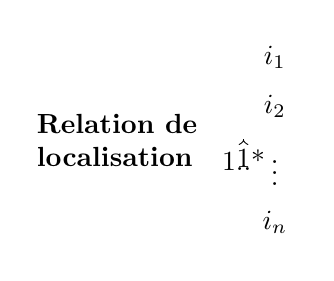
\begin{tikzpicture}
  \tikzset{
    acc/.style={decorate,decoration={brace,raise=0cm,amplitude=.1cm}},
    accm/.style={acc,decoration={mirror}},
    acc3/.style={acc,decoration={amplitude=.2cm}},
    acc3m/.style={acc3,decoration={mirror}}
  }
  
%% Matrices
\node[font=\bfseries, baseline, text width=2.5cm] (I) at (0,0) {Relation de localisation};

\matrix [matrix of math nodes,row sep=0.1cm,column sep=0.1cm,
anchor=west, nodes={anchor=base, baseline}] (is) at (I.east)
{i_1\\i_2\\\vdots{}\\i_n\\};

\draw[->, black] (I.east) -- (is.west) node[pos=0,below] {1} node[pos=1,below]{1..*};

\end{tikzpicture} 
  \caption[Structure générale d'une ontologie de
  décomposition]{Concepts et relations nécessaires à la définition
    d'une ontologie permettant de décomposer une \emph{relation de
      localisation} ($rl_i$) en un ensemble de \emph{relations de
      localisation atomiques} ($rla_i$).}
  \label{fig:onto_min_struct}
\end{figure}


La \autoref{fig:onto_min_struct} présente un aperçu de l'organisation
globale de l'ontologie des règles de décomposition. Comme nous
l'indiquions précédemment, les liens de décomposition partent toujours
d'une \emph{relation de localisation} et peuvent aboutir à une autre
\emph{relation de localisation} ou à une \emph{relation de
  localisation atomique.} La décomposition peut aboutir à autant de
\emph{relations} que souhaité, mais une \emph{relation de
  localisation} ne peut pas avoir de décomposition concurrentes. Les
deux ensembles de \emph{relations} (atomiques ou non) ne doivent pas
contenir de doublous.

Pour construire la base des relations de localisation, des relations
de localisation atomiques et des relations de décomposition en tre ces
deux ensembles nous avons adopté, conformément au principe
d'intégration dans le contexte métier, une démarche centrée sur le
besoin de l'utilisateur, \ie fondée sur la définition préalable des
\emph{relations de localisation.} Ainsi les relations de localisation
atomiques et les relations de décomposition sont définies
ultérieurement, par rapport aux relations de localisation et non
l'inverse, ce qui pourrait conduite à la définition de concepts
inadaptés à notre contexte applicatif.  En procédant de la sorte nous
garantissions que les concepts mis à disposition des utilisateurs
correspondent à la réalité du contexte applicatif. Pour mettre en
place cette démarche, il est nécessaire d'identifier les
\emph{relations de localisations} utilisées dans notre contexte et les
spécificités de leur usage.

%%% Local Variables:
%%% mode: latex
%%% TeX-master: "../../../../main"
%%% End:
